
\documentclass[11pt]{book}

\usepackage{amssymb}
\usepackage[utf8]{inputenc}
\usepackage{xcolor}
\usepackage{amsmath}
\usepackage{graphicx}
\usepackage{hyperref}
\usepackage{enumitem}


\makeatletter
\renewcommand*{\contentsname}{\Large Contents}

\usepackage{caption,subcaption}
\usepackage{wrapfig}

\usepackage{tocstyle}
\usepackage{tocloft}

\setlength{\cftaftertoctitleskip}{1em}
\setlength{\cftbeforetoctitleskip}{0em}

\captionsetup[figure]{font=footnotesize,labelfont=footnotesize}


\newcommand{\chapterauthor}[1]{%
  {\parindent0pt\vspace*{-25pt}%
  \linespread{1.1} \scshape#1%
  \par\nobreak\vspace*{35pt}}
  \@afterheading%
}
\makeatother
\usepackage[style=numeric-comp,sorting=none,useprefix,backref=true,hyperref,backend=bibtex,block=ragged]{biblatex}
\addbibresource{bibl.bib}


\begin{document}
\chapter{Slicing for 5G Cellular Networks}
\chapterauthor{Author Name (M. Pagin)}

\tableofcontents

\section{Introduction}

In the near future mobile networks will face numerous technical challenges due to the ever-increasing service requirements both from the users perspective (such as throughput, reliability, latency, availability) and from the Internet Service Providers point of view (in terms of operational optimizations such as cost and energy efficiency)~\cite{rost2017network}. This upsurge of network demands results from the simultaneous increase of mobile terminals, their growing diversity of requested services and the rapid evolution of new application scenarios such as inter-vehicular communication, Internet Of Things, Industry 4.0 and the Smart City concepts \footnote{Such scenarios are usually subdivided into three categories, summarized in Fig.~\ref{Fig:5g-req}}. It follows that the new generations of mobile networks must then meet the following contrasting goals: the fullfillment of the aforementioned service requests and, at the same time, the avoidance of strategies involving deployments of singular mobile network solutions for every use case; in particular, the latter becomes strictly necessary in order to provide cost and energy-efficient solutions and a design which aims to be as future-proof as possible. For these reasons, the upcoming network designs need to be scalable and flexible, two fundamental requirements which play a key-role in the insurance of the adaptability of the mobile network to the specific scenario that the various use cases present. As an example of the plethora of different technical requirements that these extremely heterogeneous use cases require, packet error rates of $10^{-4}$ are tolerable in a mobile broadband system; however, when it comes to industrial real time applications, typical target values for the aforementioned metric are in the order of $10^{-9}$, since such scenarios require extremely high reliability and must also meet strict latency constraints~\cite{frotzscher2014requirements, parvez2018survey}.
\begin{figure}[!ht]
    \centering
    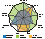
\includegraphics[scale=11]{figures/5g-req.pdf}
     \setlength\belowcaptionskip{.1cm}
  \caption{Key 5G use cases and their requirements. In this illustration, the further the distance of a requirement from the center, the more important it is to the corresponding use case. It is inspired by a similar illustration from ITU ~\cite{ITU}.}
    \label{Fig:5g-req}
\end{figure}

Network Slicing, defined by the \textit{Next Generation Mobile Networks} (NGNM) alliance as the concept of running multiple logical networks as independent flows upon a common physical infrastructure, is the main proposed solution to meet the above-mentioned requirements. Specifically, a network slice is a self-contained, virtualized and independent end-to-end network that allows operators to execute different deployments in parallel, each one based on its own architecture~\cite{alliance2016description}; a network slice is also capable to offer customized functionalities, including those in the UE, and delivers services to each device using network function chains. Furthermore, Network Slicing is an abstract concept that can be actually implemented by employing ad-hoc network architectures both at the \textit{Core Network} (CN) and at the \textit{Radio Access Network} (RAN): our focus will be on the latter, but a general overview of both cases will be presented nevertheless. 
It must be also noted that the aforementioned concept reflects one of the main principles of the overall design philosophy of 5G Cellular Networks: one of its general trends is the virtualization of the network components and the aim to provide a modular and flexible design; specifically, in such regard, two fundamental technologies enablers are identified within the concepts of \textit{Network Function Virualization} (NFV) and \textit{Software Defined Networking} (SDN)\cite{yousaf2017nfv, kaloxylos2018survey}. 
\begin{figure}[t]
    \centering
    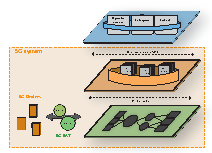
\includegraphics[scale=3.65]{figures/NFV.pdf}
     \setlength\belowcaptionskip{.1cm}
  \caption{Key 5G use cases and their requirements. In this illustration, the further the distance of a requirement from the center, the more important it is to the corresponding use case. It is inspired by a similar illustration from NGNM ~\cite{alliance2015description}.}
    \label{Fig:NFV}
\end{figure}
The first term refers to the paradigm shift of moving the various networking-related functions from dedicated hardware to software solutions running on top of Virtual Machines, hence allowing a modular architecture and flexibility on the placement of such Virtual Functions, effectively enabling the introduction of an API-like framework. Unfortunately, in order to reach an effective deployment of these technologies in mobile network some open-challenges still need to be faced.
On the other hand, the major contribution of the latter is an evolved separation between control and user planes: such goal has already been partially pursued by previous 3GPP specifications~\cite{3gpp_LTE} with the introduction of the \textit{Evolved Packet Core} (EPC), but such implementation kept a certain degree of inter-connection between the planes which is now abandoned thanks to the NFV abstraction. It is then clear that these enablers (whose high-level architecture can be seen in Fig.~\ref{Fig:NFV}) are built on top of one another and their co-existence is vital in order to provide a programmable and agile network structure, which in turn effectively allows the introduction of the Network Slicing concept. 

The purpose of this chapter will then be to introduce the aforementioned concept and to highlight the very same design changes that allow its envision. Specifically, the concepts of NFV and SDN will be first introduced (following what has been, up to a certain degree, the research focus timeline), followed by an explanation of how such technologies enable Network Slicing. Finally, some purposed architectures and solutions will be presented, with an in-depth analysis of a RAN, multi-connectivity based approach.

\section{Enablers: NFV and SFN}
\subsection{Network Function Virtualization}
As previously mentioned, the term \textit{Network Function Virtualization} (NFV) refers to a paradigm shift towards the employment of software-based solutions, running on top of virtual machines. This revolution is driven both by the rapid rise in the computational power of generic-purpose hardware and the success of cloud-based solutions, effectively leading to the will of virtualizing network components such as firewalls, routers and even the whole EPC, whose historical and current implementations rely upon dedicated hardware technologies. Such innovations open the possibility of using automated tools derived from the cloud infrastructures to manage and orchestrate the network, operations that are currently undertaken semi-manually, hence providing promising cost reductions benefit; on top of this, NFV also paves the way for a shift from the telco's ``hardware that can't fail" paradigm to the high-availability concept of the cloud world, that instead aims to partition the system in order to limit single points of failure. Finally, another benefit of this virtualization is the decoupling from the slow release cycle of the dedicated hardware commodities to the possibly agile deployment of new and updated software solutions and configurations~\cite{yousaf2017nfv}.

Initially, the transition from monolithic hardware to virtualized solutions has taken place by means of porting the formers to massive virtual machines appliances, each representing a \textit{Virtual Network Function} (VNF); in turn the latter are grouped together by \textit{Service Function Chains} in order to constitute a \textit{Network Service}. Even though this naive software porting already introduced tangible benefits in the form of flexibility and management, as it allowed the usage of cloud-derived automation tools and the possibility of introducing the high-availability concept using redundant systems, this approach has been deemed (e.g. in~\cite{taylor2015}) to be too ``telco's centric" and to not being able to fully exploit the advantages that a cloud centric design can bring. This initial failure was caused by the fact that a straightforward porting is not capable to deliver the same performance that dedicated hardware solutions can, especially on standard cloud environments that actually introduce significant overhead, limiting the performance of delay sensitive applications. Additionally, such solutions lack the capability to scale well with respect to the network demands, since they hardly allow the dynamic addition or removal of computing nodes. These problems have been solved by adapting a more radical shift towards native cloud solutions, specifically by developing network functions with a much smaller footprint, running on slim containers (instead of big virtual machines) and allowing cloud-like scalability.
Unfortunately though, nothing comes for free: this is no exception as this modular, cloud native design also brings the disadvantages that the management of such a complex solution introduces: orchestrating a massive amount of slim and inter-operating NFV entities is not trivial at all. Therefore, such role required the introduction of another new entity, the so called \textit{Management and Orchestration} (MANO) system, whose purpose is the simplified handling of complex network services employing the NFV technology. In order to do so, MANO systems must attend to the management of the various virtualized, cloud and network infrastructures, the organization of the different NFV entities and regulation of their life cycles. Moreover, referring once again to Fig.~\ref{Fig:NFV}, the interaction between the three presented layers must be managed, as well as the orchestration of the various virtual and physical resources, with the aim to fully exploit these infrastructures.
\begin{figure}[h!]
    \centering
    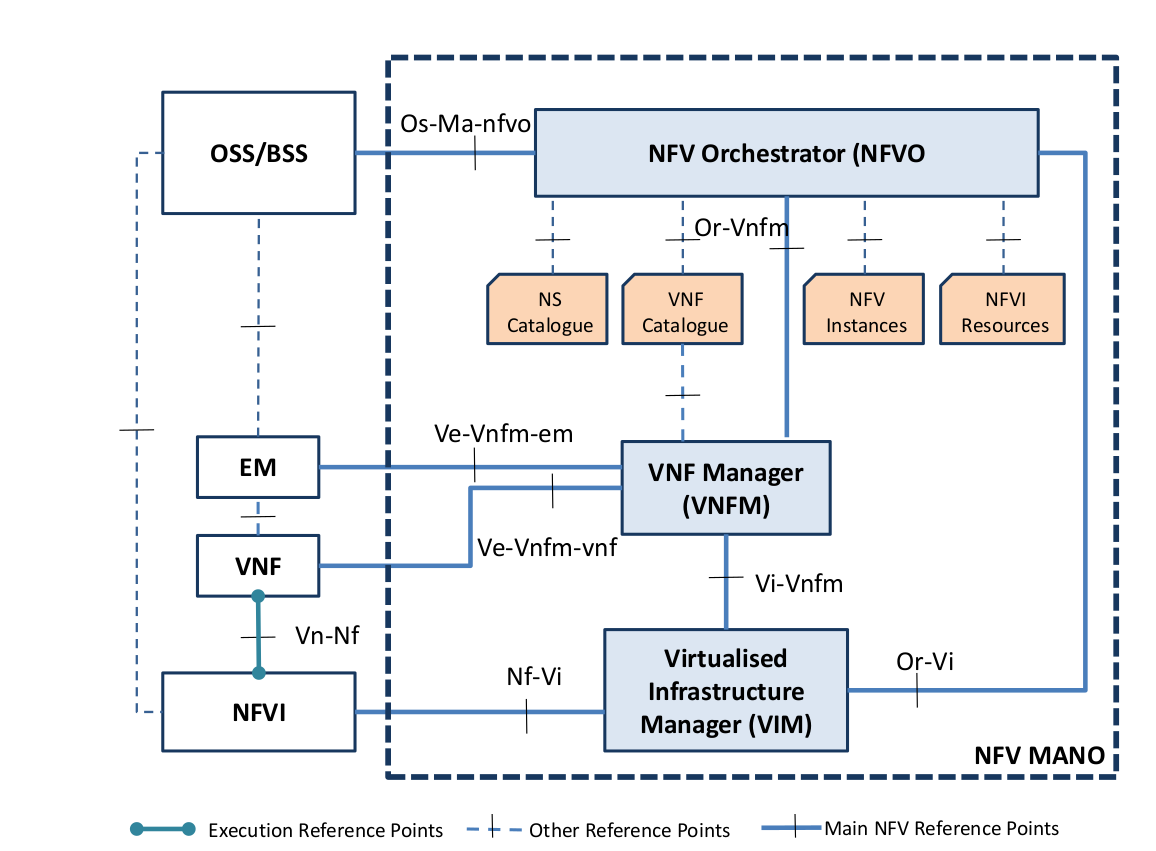
\includegraphics[scale=1.1]{figures/NFV.png}
     \setlength\belowcaptionskip{.1cm}
  \caption{Placeholder}
    \label{Fig:NFV_MANO}
\end{figure}
As of today, the most relevant NFV MANO framework is the reference model specified by ETSI~\cite{etsiSpec} and depicted in Fig.~\ref{Fig:NFV_MANO}. This framework is composed of three main functional blocks, namely the \textit{Virtualized Infrastructure Manager} (VIM), the \textit{Virtual Network Function Manager} (VNFM) and the \textit{Network Function Virtualization Orchestrator} (NFVO). These entities operate in the following hierarchical manner: the VIM manages the NVF at the virtual machine level, by interacting with the cloud infrastructures; the VFNM manages, on top of the previous layer, the life cycle operations of the single VNFs (such as their scaling and configuration) and finally, the NFVO manages the various network services, which in turn are composed of an aggregation of NFVs~\cite{yousaf2017nfv, etsiSpec}.
\subsection{Software Defined Networking}
In a certain way, \textit{Software Defined Networking} (SDN) is, just like MANO, a concept whose envision is driven by the need to manage, even though at a different level, the complexity that the NFV concept introduces: for example, the network infrastructure might possibly need to be re-configured on a regular basis in order to support the NFV architecture. Such operation is though quite tedious to perform on legacy systems and requires manual\footnote{Almost, or at least semi-manual in most of the cases~\cite{yousaf2017nfv}} intervention, hence it usually works over pretty long time scales (such as hours or even days): this is a clear limitation of traditional network designs and SDN has been designed with the very same goal of overcoming such problems. Specifically, SDN consists in the paradigm shift towards making networks programmable and enabling applications and network services to directly control the abstracted infrastructure; the means to obtain such goal are the substitution of the plethora of proprietary equipment and services with a set of deeply programmable and common software-driven services and methods that span across multiple vendor-platforms \footnote{We hereby recall that the next generation of mobile networks are envisioned to offer support for multi-tenancy solutions}. 
A protocol of particular importance within this realm is OpenFlow, whose aim is  to regulate the inter operability of network infrastructure elements and the network controlling, software-based entities. As in previous cases we delegate a detailed description of such protocol to~\cite{yousaf2017nfv, onfSpec}, limiting ourselves to a simple enunciation of its basic principles, namely:
\begin{itemize}[noitemsep, topsep=0.2pt]
\item the decoupling of control and user planes. Such concept allows the independent deployment and life cycles regulation of traffic forwarding and processing entities.
\item the deployment of a centralized control unit. Furthermore, such control appears from the outside, application perspective as a single entity, but it is not actually required to be deployed as a centralized monolithic implementation.
\item the programmability of network services. Interfaces between the various SDN components shall expose their resource abstractions and applications should be enabled to act on the latters by programmatically exploiting a well defined API.
\end{itemize}
\section{The birth of 5G Network Slicing}
The aforementioned enablers effectively introduce the support for the Network Slicing concept, namely an end-to-end virtualized environment, abstracted from the underlying hardware technologies and which promises to support the tailoring of their control to the different slices service requirements in a programmatic manner via APIs. Moreover, its novelty factors lie in the exposure of such control to verticals (and third parties in general), the flexibility that it promises to deliver and its end-to-end nature, characteristics that make it differ from the previously purposed solutions~\cite{rost2017network}.


A concrete example of how the above-mentioned technologies can be exploited within this realm is given by the 5G NORMA project, envisioning the following scenario~\cite{normaSpec}: the various slices operate on top of an infrastructure composed of both generic hardware resources (namely, VNFs) and dedicated solutions such as RAN network elements; furthermore the formers make up a set of common NFs which get shared by the overlying slices, while the latters form dedicated and ad-hoc designed sub-slices. The management of these entities is then delegated to a couple of software-defined controllers: the SDM-C, whose role is the orchestration of the dedicated sub-slices and the SDM-X, undertaking the more complicated management of the shared pool of resources (see Fig.~\ref{Fig:SDN}). 
\begin{figure}[h!]
    \centering
    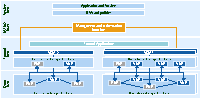
\includegraphics[scale=3.95]{figures/SDN.pdf}
     \setlength\belowcaptionskip{.1cm}
  \caption{The design envisioned by the 5G NORMA project~\cite{normaSpec} for the co-existence of SDN and NFV as Network Slicing enablers, merging dedicated and shared sub-slices to form end-to-end mobile network instances. The illustration is inspired by a similar one exhibited in~\cite{rost2017network}}
    \label{Fig:SDN}
\end{figure}
Specifically, the latter shall face the challenge of providing a dynamic, inter-slice scheduling of the RBs in order to grant an agile and flexible adaptation to the channel conditions and thus satisfy the slice' QoS requirements; on the other hand the idea of designing an SDM-X assigning resources in a static manner has been sidelined, as such approach would result in an inefficient network utilization (and would not fully exploit the potential of SDN and NFV), even though it would exhibit an always welcome lower design complexity.
\subsection{An end-to-end approach}
Previously it has been stressed that Network Slicing is, by design, envisioned to have an end-to-end span: therefore, it follows that solutions both at the CN and RAN must be introduced; the nature of such implementations to be substantially different as a result of their vastly heterogeneous characteristics. Regarding the CN, its structure and its dependency on generic purpose hardware allow for an high degree of exploitation of the SDN and NFV concepts, since most of its functions can be easily virtualized and therefore centralized. Moreover, the purposed CN design consists in the breaking down of the various network functions into smaller and lighter sub-modules that are to be re-grouped and possibly shared by the higher level VNFs~\cite{An2017ArchitectureMF}. Additionally, the aforementioned enablers will also allow the decoupling of user and control planes, thus supporting a centralized implementation of the latter which can then be exposed to third parties, hence providing cloud-like scalability and multi-tenancy support~\cite{5gCrosshaul}.

Conversely, the RAN functions exhibit tight coupling with the underlying dedicated and efficient hardware, which is basically necessary in order to withstand strict execution time constraints, hence making the design of a centralized and fully virtualized solution almost unfeasible and definitely sub-optimal~\cite{kaloxylos2018survey}. Therefore, even though some small portions of the RAN can still be virtualized, the majority of the Network Slicing implementations are limited to a customized configuration of the RAN parameters, which is still enough to grant a management of the radio resources capable to satisfy the slices' QoS requirements. Specifically, two classes have been identified in such regard: time-\textit{asynchronous} ones \footnote{With respect to the radio interface} as LTE's PDCP and RRC layers functions and time-\textit{synchronous} ones like RLC layer downwards functions; the former class, requiring low data rates and scaling just with the number of connected users, is well suited to the VNF concept, on the other hand the latter exhibits performance requirements which do not bode well with such approach. Therefore, in the aforementioned cases a centralized solution is to be preferred only in specific instances, while in the remaining ones the favored solution is to keep the dedicated hardware design, with the addition of its custom, slice-specific (and possibly, SDN controlled) configuration~\cite{marsch20165g}. As an example of such, the RAN protocol stack can serve a slice requesting high throughput such as \textit{Enhanced Mobile Broadband} (eMBB) by employing multi-connectivity (MC) techniques, as well as set-up \textit{Multiple Input and Multiple Output} (MIMO) to offer multiplexing gain; conversely slices requiring very low latency like \textit{Ultra Reliable and Low Latency Communications} (URLLC) may leverage the latter for delivering improved error resilience and exploit ad hoc MAC layers HARQ techniques. 


Even though the portion of RAN functions which are envisioned to offer slice-specific adaptation is still an open research topic, it is likely that the co-existence of more than one design will take place, with the network offering the capability of choosing among them in order to tailor the design to the possible slices demands. In particular, the 5G NORMA project~\cite{normaSpec2} presents three such options, namely:
\begin{enumerate}[noitemsep, topsep=0.2pt]
\item \textit{Slice-specific RAN.} The first option of Fig.~\ref{Fig:RANArchi} consists in limiting the common functions to the transmission point ones only, instantiating the rest of the network in a slice-specific manner. It is the design promising the higher degree of freedom regarding the adaptability to the slice characteristics, but on the other hand such fragmentation possibly limits the effectiveness of joint optimization strategies, thus missing out on multiplexing gains.
\begin{figure}[!ht]
    \centering
    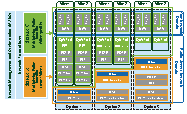
\includegraphics[scale=3.95]{figures/RANArchi.pdf}
     \setlength\belowcaptionskip{-.1cm}
  \caption{Three possible RAN Slicing architectures purposed by the 5G NORMA project. The illustration is inspired by a similar one exhibited in~\cite{normaSpec2}}
    \label{Fig:RANArchi}
\end{figure}
\item \textit{Slice-specific radio bearer.} Option 2 of Fig.~\ref{Fig:RANArchi} presents a reasonable trade-off between network complexity and adaptation capabilities. It depicts a shared PHY, MAC and RRC implementation, hence providing both a less complicated design and decent customization capabilities, as the slices still have the chance of dictating custom configurations of the lower levels and to possibly implement their ad hoc QoS control strategies.
\item \textit{Slice-aware shared RAN.} The final option presented in Fig.~\ref{Fig:RANArchi} refers to a completely shared RAN, offering as only customization possibility the tailoring of the SMD-X parameters.
\end{enumerate}


Finally, it is important to stress once again that the Network Slicing concept relies on the novel flexibility that 5G introduces: specifically, in the RAN realm the so-called radio tiling allows the radio resources to be efficiently and appropriately shared among the different slices, in a manner which was simply not possible with LTE and older specifications.

\section[The upcoming RAN revolution]{The upcoming RAN revolution: further enablers and their Network Slicing exploitation}
In addition to the flexibility introduced by the technologies that have been previously presented in this chapter, further changes must be implemented in the RAN in order for the upcoming mobile networks to face their ever-increasing traffic demands; in this section some of these technologies are going to be introduced, namely \textit{Multi Connectivity} (MC) and \textit{milliMiter wave} communications (mmWave), along with a Network Slicing design implementing them.
\subsection{Enablers: CA and mmWave}
In the context of new generation mobile networks, it is envisioned that UE terminals will be able to connect to multiple eNBs: specifically, RAN MC refers to the support for the co-existence of multiple UEs connections to different PHY interfaces, which are leveraged to offer higher throughput capabilities or improved error resilience. Similarly to the above-mentioned technologies, MC can be implemented at different layers of the RAN protocol stack, each providing its own complexity/capabilities trade-off~\cite{rost2017network}; in particular the 3GPP New Radio (NR) specifications presents the following MC designs: \textit{Carrier Aggregation} (CA) for single-RAT solutions and Dual Connectivity (DC) for both single and multi-RAT approaches~\cite{3gppSpec, Zugno_2018}. The former refers to a MAC layer MC implementation, which uses the multiple links (the so-called \textit{Carrier Component}s (CC))  to transmit different data streams, possibly at different frequencies and with custom MAC and PHY layers configurations (such as tailored retransmission processes, MCS and so on..). 
%Such technique has already been used in LTE-A networks, providing both throughput enhancements and agile interference management \cite{pedersen2011carrier}.
Conversely, DC implements MC by offering UEs the possibility of connecting to multiple cells, integrated at the PDCP layer~\cite{3gppSpec2} and having independent lower layers. Even though the latter allows, conversely from CA, to connect to non co-located base stations it also offers a lower degree of freedom: since the RLC layers are bearer-dedicated, once the data is committed to one of them that choice can not be reversed, on the other hand CA allows joint scheduling at the MAC layer across the different CCs (since each bearer shares the same RLC layer instance for all of them). Finally, DC is also deemed to be promising in the multi-RAT realm, allowing solutions such as inter-networking between LTE and 5G cellular networks~\cite{Silva2015TightIO, Polese_2017}.


The scenario predicted by upcoming network traffic forecast also predicts an ever-increasing need for new radio resources: since the usual frequencies are already incredibly crowded and thanks to advancements in the hardware technologies, the interest has shifted towards the exploitation of mmWave frequencies, namely the portion of the radio spectrum above 6 GHz.  The massive amount of currently unused bandwidth that mmWave frequencies promise to offer counterbalances the harsh propagation characteristics that this portion of the spectrum exhibits: specifically,  high isotropic path loss and blockage susceptibility are the main antagonists in such regard~\cite{rangan2014millimeter}. Nevertheless, such challenges can be overcome by using dense network deployments~\cite{rangan2014millimeter} and leveraging the high antenna directionality that these frequencies exhibit, on top of the possibility of packing multiple antenna elements in relatively small components~\cite{sun2014mimo, roh2014millimeter}.

\subsection{Achieving RAN slicing through CA in mmWave cellular networks}
The novel Network Slicing implementation that we hereby introduce is based on both the aforementioned enablers: namely, we present a possible exploitation of CA at mmWave frequencies for Network Slicing. The will to inspect the effectiveness of such marriage is driven by the fact that these two technologies seemingly complement one another, each one of them offering a solution to its colleague weaknesses. 


\begin{wrapfigure}{l}{0.57\textwidth}
  \begin{center}
    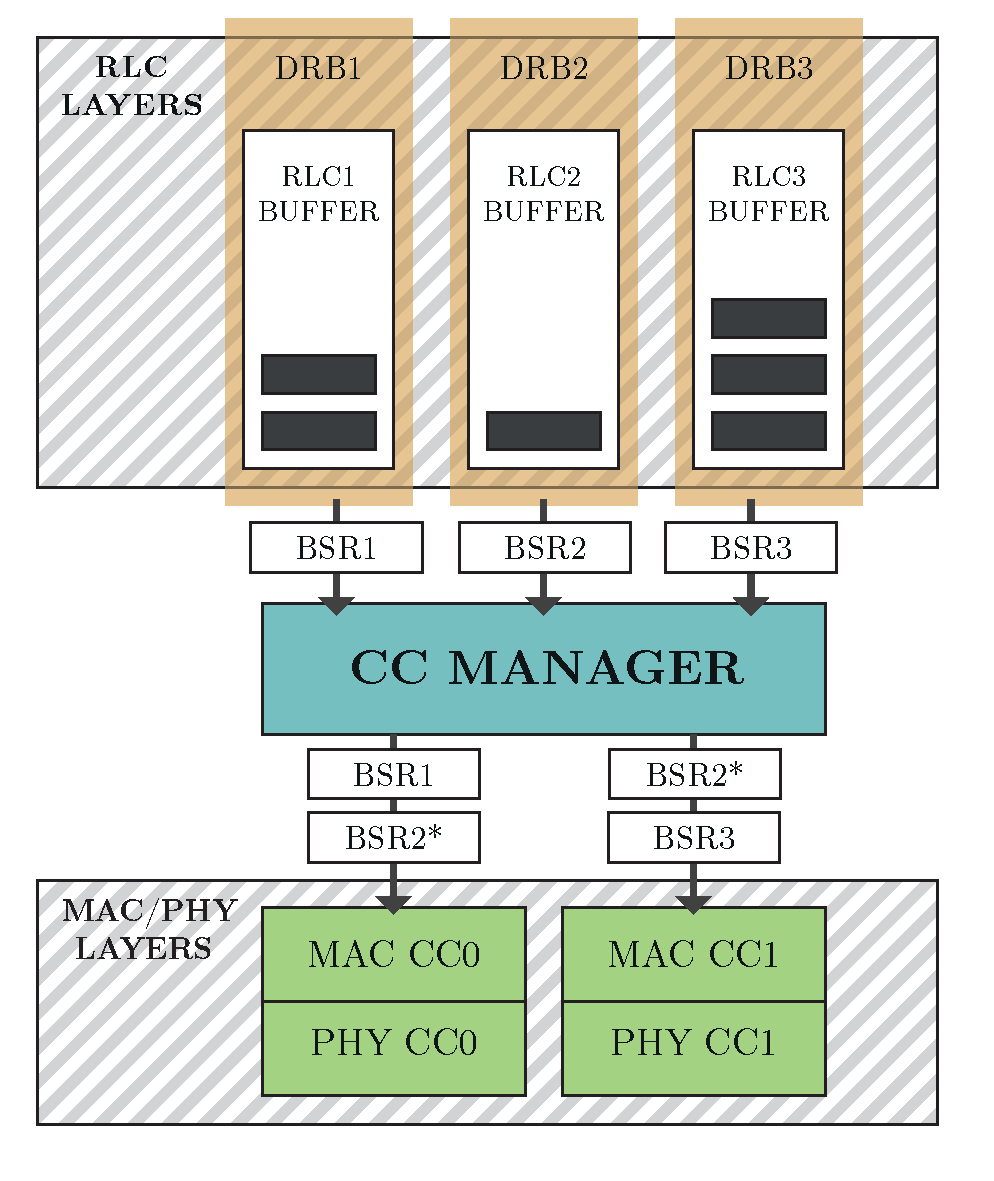
\includegraphics[width=0.54\textwidth]{figures/stack-figure.pdf}
  \end{center}
  \caption{Protocol stack of a NR, CA system. In~\cite{pagin2020} the BSR messages incoming from the above RLC layers get redistributed across the various CCs, possibly depicting different amount of data compared to their original form (see BSR2 and BSR2*)}
  \label{Fig:Stack}
\end{wrapfigure}
Specifically, mmWave frequencies suffer from blockages and high path loss, in such regard the MC provided by CA can be exploited to offer higher reliability and to aggregate the available bandwidth to offer even more throughput; on the other hand CA can exploit the aforementioned portion of the radio spectrum as a mean to find idle bandwidth, which would otherwise be difficult to enjoy in the crowded frequencies used in previous generations of mobile networks. Finally, all of the above can clearly serve as a Slicing enabler, by tailoring the service offered by CA and mmWaves to the slice specific QoS requirements.

\subsubsection{Slice-aware scheduling}
The approach purposed in~\cite{pagin2020} envisions a RAN Slicing implementation located between the RLC and the MAC layers, leveraging an intermediate entity called \textit{Carrier Component Manager} whose role is to provide inter-CC scheduling to the layers above. Specifically, as can be seen in Fig.~\ref{Fig:Stack}, the envisioned design dictates the RLC layers (one for each radio bearer) to forward their \textit{Buffer Status Report}s (BSRs) to the CC Manager, which in turn shall re-shuffle them across the available CCs, trying to tailor such choice to the flow specific demands. Morevoer, the case of co-existing eMBB and URLLC vastly heterogeneous slices has been studied, the former exhibiting massive throughput demands and the latter requiring extremely strict latency and reliability constraints. Within such realm, the following heuristic scheduling strategy has been purposed: each flow gets associated to a primary, most suitable carrier that is to be predominantly used, while the remaining, less preferable ones shall be exploited only if the flows favoring such carriers do not have too much data to transmit.
\begin{figure}[t]
  \begin{center}
    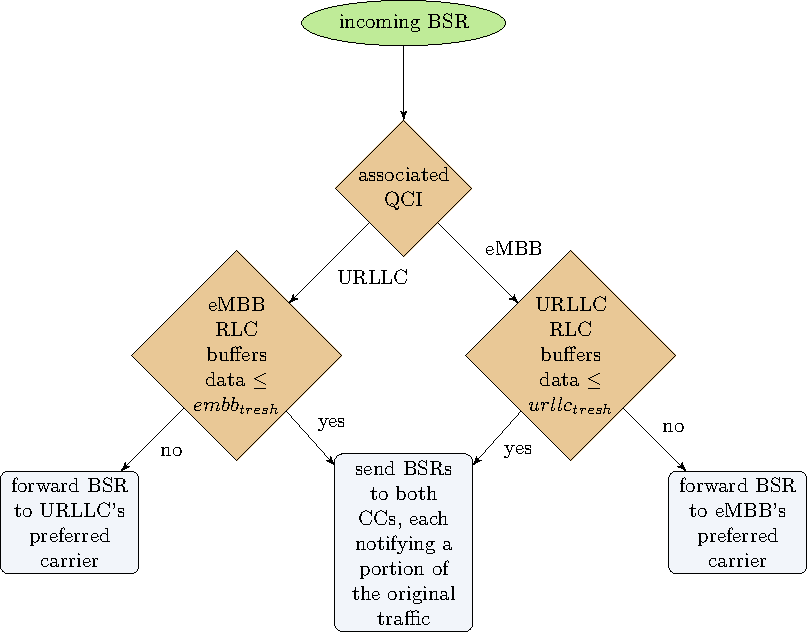
\includegraphics[width=0.65\textwidth]{figures/algo-flow-chart.pdf}
  \end{center}
  \caption{Flow-chart of the BSR scheduling logic}
  \label{Fig:FlowChart}
\end{figure}
In particular, in the aforementioned case of URLLC and eMBB traffic sources the data is spreaded across the CCs by following this simple criteria: URLLC traffic shall be partially redirected towards its non-preferred CC if and only if the eMBB RLC buffers contain less data to transmit than a pre-determined threshold $\mathrm{embb_{tresh}}$; the same holds for the eMBB traffic, by reversing the respective roles in such explanation (see Fig.~\ref{Fig:FlowChart}).
\subsubsection{Simulation-based performance analysis}
The aforementioned scheduling policy has then been implemented in ns3, an open-source discrete-event simulator capable of performing accurate end-to-end simulations, in order to evaluate its effectiveness. In particular, the mmWave~\cite{mmwave5gmodule} module, integrated with its 3GPP MIMO channel~\cite{mmwave3gppchannel} and CA~\cite{Zugno_2018} extensions has been employed, extending the latter in order to implement the purposed solution \footnote{For a detailed explanation of such implementation we kindly refer to reader to~\cite{pagin2020}. Nonetheless, for the presented, brief treatment of the matter Fig.s~\ref{Fig:Stack} and~\ref{Fig:FlowChart} shall suffice.}. This RAN Network Slicing implementation has then been tested by simulating an urban, densely populated scenario consisting of a single serving base-station, surrounded by terminals equipped with \textit{User Datagram Protocol} (UDP) applications receiving either eMBB or URLLC traffic; moreover, such UEs move within a predetermined area according to a bi-dimensional random walk. Regarding the carriers choice, it has been chosen to assign to the URLLC primary CC a central frequency of 10 GHz, while 28GHz has been picked for the eMBB slice: the reasoning behind such decision is that the isotropic path loss increases with the square of the frequency, hence the former should provide the URLLC reliability and delay requirements in a more effective manner compared to the eMBB's depicted CC.

The effectiveness of the purposed solution has been analyzed by means of simulation, focusing on the evaluation of the slices predominant QoS KPIs, namely delay for URLLC and overall throughput for eMBB; additionally a spectrum efficiency metric $\eta_{spectrum}$ has been introduced, measuring the ratio of PHY symbols transmitted over the available ones. 

\begin{wrapfigure}{L}{0.58\textwidth}
  \begin{center}
    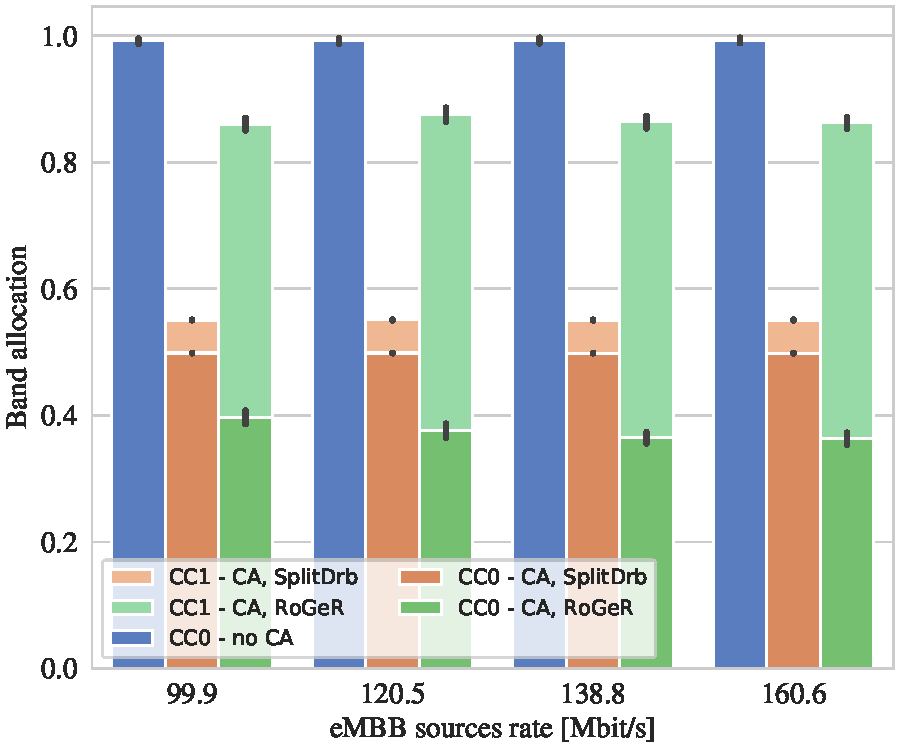
\includegraphics[width=0.55\textwidth]{figures/Band_allocation_eMBB_rate.pdf}
  \end{center}
  \caption{$\eta_{spectrum}$ for eMBB sources rate varying $\in$ $[100, 120. 140, 160]$ Mbit/s, URLLC data-rate fixed at $1.5$ Mbit/s}
  \label{Fig:Band}
\end{wrapfigure}
In particular, the aforementioned metrics have been employed in order to benchmark the solution purposed in~\cite{pagin2020} against the following strategies: not using CA at all and using it to provide flow orthogonalization, namely a static association between CCs and slices. As can be seen in Fig.~\ref{Fig:Band}, the first take-over from such analysis is that the latter strategy fails to fully exploit the available system bandwidth: reserving the CCs for a specific slice is definitely inefficient and, in the case of eMBB, does not even provide significant performance benefits; such outcome can be explained by the fact that a fixed bandwidth resources allocation is not capable to adapt to the flows different rates, on top of missing out on any multiplexing gain that CA can offer. Finally, the effectiveness of this Network Slicing strategy can be also appreciated in Fig.~\ref{fig:Perf}, depicting the predominant system KPIs as the number of users varies in $[5, 10, 15]$: the system, when using RoGeR, exhibits both the capability to adapt to the eMBB throughput demands and almost no susceptibility with respect to variations of the amount of URLLC users, showing no performance degradation as such value increases.
\begin{figure}[t]
  \centering
  \begin{subfigure}[t]{\columnwidth}
    \centering
      \setlength\belowcaptionskip{.1cm}
    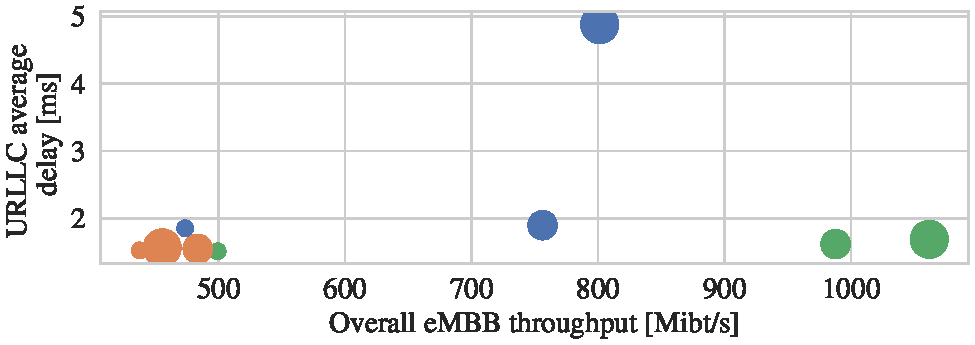
\includegraphics[width=0.65\textwidth]{figures/Throughput_vs_delay_numEmbbUes.pdf}
    \caption{URLLC average APP layer delay versus overall system eMBB APP layer throughput.  Each marker size is proportional to the amount of eMBB sources, varying in $[5, 10, 15]$.}
    \label{fig:PerfNumEmbb}
  \end{subfigure}
  \begin{subfigure}[t]{\columnwidth}
    \centering
    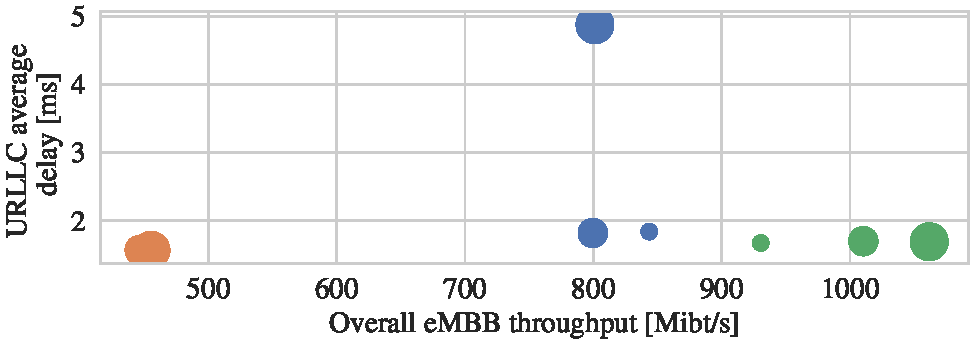
\includegraphics[width=0.65\textwidth]{figures/Throughput_vs_delay_numUrllcUes.pdf}
    \caption{URLLC average APP layer delay versus overall system eMBB APP layer throughput.  Each marker size is proportional to the amount of URLLC sources, varying in $[5, 10, 15]$.}
    \label{fig:PerfNumUrllc}
  \end{subfigure}
  \setlength\belowcaptionskip{-.5cm}
  \caption{System performance summary, as the number of eMBB and URLLC sources varies $\in$ $[5, 10, 15]$}
  \label{fig:Perf}
\end{figure}
Therefore, such solution shows that the employment of CA at mmWave frequencies for Network Slicing is indeed promising, and in such regard further analysis, coupled with the design of optimal inter-CC schedulers promises to provide interesting results.

\section{Conclusions}
In this chapter the concept of Network Slicing has been presented, introducing its enablers and explicitly mentioning its role within the next generation of mobile networks. Moreover, some Network Slicing implementation considerations have been presented, introducing CN and RAN possible designs, but focusing mainly on the latter. Finally, the most promising innovations within the RAM that upcoming mobile networks will bring have been introduced, describing how such technologies can be exploited to offer Network slicing solutions, both in a generic manner and by presenting a specific RAN Network Slicing design.





\addcontentsline{toc}{section}{References}
\printbibliography

\end{document}